\part{Arduino}
\chapter{Arduino}\label{analysis:arduino}
Arduino was created by the Interaction Design Institute Ivrea (Italy), by Massimo Banzi and David Cuartielles. They were looking for an easy and cheap way for students, who study design, to integrate micro controllers into their projects\cite{arduino:hist}. Both the board and the programming language was based on the works of Hernando Barragán, one of Massimo Banzi master thesis students \cite{Wiring:thesis}.

In this project Arduino board is used to execute the code, and show a type of output. The output will be in the form of a LCD Display. 

\section{The Hardware Components}
Arduino is a single-board micro-controller, see figure \ref{fig:Arduino_uno}.
A board consists of open source hardware, which is designed around an 8-bit Atmel AVR micro-controller. Arduino boards varies in sizes. Arduino Uno board for example, has a max width of 2.1'' (5,33cm) and a length of 2.7'' (6,86cm).  \\

\par
\raisebox{-.5\height}{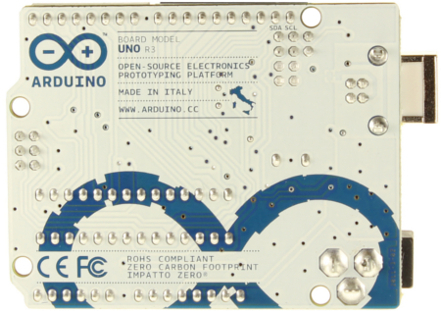
\includegraphics[width=6.5cm]{billeder/ArduinoUno_R3_Back_450px.jpg}}
\hfill
\raisebox{-.5\height}{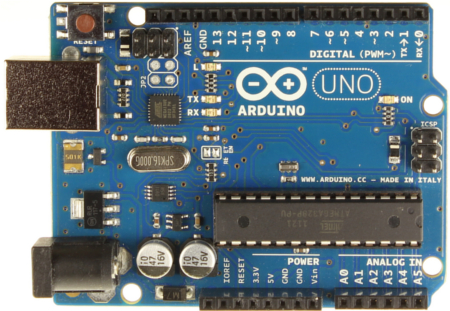
\includegraphics[width=6.5cm]{billeder/ArduinoUno_R3_Front_450px.jpg}}
\begin{figure}[H]
\caption{Picture of back- and fronside of the Arduino Uno board \cite{Arduino:board_pics}}
\label{fig:Arduino_uno}
\end{figure}
\par

\par
\raisebox{-.5\height}{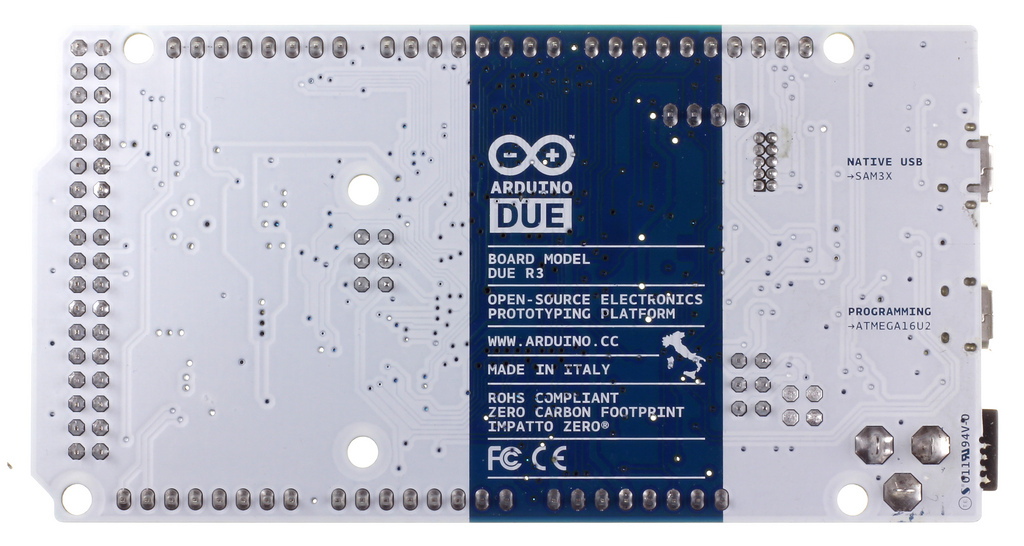
\includegraphics[width=6.5cm]{billeder/ArduinoDue_2.jpg}}
\hfill
\raisebox{-.5\height}{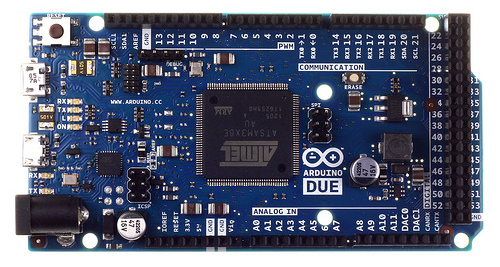
\includegraphics[width=6.5cm]{billeder/ArduinoDue_1.jpg}}
\begin{figure}[H]
\caption{Picture of back- and fronside of the Arduino Duo board \cite{Arduino:board_pics}}
\label{fig:Arduino_duo}
\end{figure}
\par

\subsection*{Specifications}
The board provides some input and output possibilities. The Arduino Uno, figure \ref{fig:Arduino_uno}, has 14 digital I/O and 6 analog inputs, where as the Arduino Due, figure \ref{fig:Arduino_duo}, has 54 digital, and 12 analog pins. The I/O functions are placed on top of the board, and are freely accessible, and consist of 0.1'' female headers. Besides the I/O there is also a Power connector, which almost in all cases require 5 volt DC. There is an USB connection on the board, so that processing data to the micro-controller is possible, though it is shown as a virtual com-port on the connected computer. However, on older boards, instead of the USB connection, a RS232 were used for serial communication. 

\begin{figure}[H]
\centering
\begin{tabular}{|c|c|}
\hline 
Microcontroller & ATmega328 \\ 
\hline 
Operating Voltage & 5V \\ 
\hline 
Input Voltage (recommended)	 & 7-12V \\ 
\hline 
Input Voltage (limits) & 6-20V \\ 
\hline 
Digital I/O Pins & 14 (of which 6 provide PWM output) \\ 
\hline 
Analog Input Pins & 6 \\ 
\hline 
DC Current per I/O Pin & 40 mA \\ 
\hline 
DC Current for 3.3V Pin & 50 mA \\ 
\hline 
Flash Memory & 32 KB (ATmega328) of which 0.5 KB used by bootloader \\ 
\hline 
SRAM & 2 KB (ATmega328) \\ 
\hline 
EEPROM & 1 KB (ATmega328) \\ 
\hline 
Clock Speed & 16 MHz \\ 
\hline 
\end{tabular} 
\caption{Hardware specifications for the Arduino Uno}
\end{figure}

On the board there is a LED, which is connected to the digital pin 13. When this diode is set to ``HIGH'' it will be turned on, and if its value is ``LOW'' it turns off. Besides the LED, there is also a reset button. If the button is pressed the micro-controller is reset. 

The specifications, which are important to take into consideration in regard to designing a programming language aimed at the Arduino platform, is the flash memory, the main memory(SRAM) and the CPU speed. The most limiting factor to take into consideration is the amount of RAM, the larger and more complex the data structures are, the bigger the risk of running out of memory while executing a program. Although this is not limited to developing for the Arduino platform, it is certainly a larger factor, then when developing for desktop computers.
Another factor that need attention is the flash memory, meaning the pace available for the program, the smallest example code for the Arduino, the Blink example listings \ref{lst:blink}, only uses 1084 bytes, which is approximately $3.3 \%$ of the total memory available. 

\begin{table}[h!]\scriptsize
\centering
\begin{tabular}{cc} 
\begin{minipage}{6cm}
{\begin{lstlisting}[caption=Arduino,frame=none,resetmargins=true,label={lst:blink}]
int led = 13;
void setup() {                
  pinMode(led, OUTPUT);     
}

void loop() {
  digitalWrite(led, HIGH);   
  delay(1000);    
  digitalWrite(led, LOW);  
  delay(1000);
}
\end{lstlisting}}
\end{minipage}
  & 
\begin{minipage}{10cm}
{\begin{lstlisting}[caption=C\#,frame=none,resetmargins=true,label={lst:C_hello}]
namespace hello
{
  class Program
  {
    static void Main(string[] args)
    {
       System.Console.WriteLine("Hello, World!");
       System.Console.ReadKey();
    }
  }
}
\end{lstlisting}}
  \end{minipage}
 \\ 
 \end{tabular} 
 \caption{Comparison between a simple Arduino and C\# example}
 \end{table} 

If a language has a lot of complex features, it will quickly run out of space. For instance with more complex languages like C\#, a simple hello world, listings \ref{lst:C_hello}, program uses 5120 bytes, and they can quickly run in the hundreds or thousands of kilobytes. This is even more important to remember, when one takes into account, that there are many different Arduino configurations, and the language have to function on all of them. The Arduino Nano for instance, only has 16 KB of memory, and there are Arduino clones by other manufactures with even less.



\subsection*{Components}
What makes Arduino such a good platform for beginners to learn to program on, is because it is really easy to connect a wide variety of components to it, making it possible for the Arduino to interact with the real world.

\begin{itemize}
\item[] \textbf{LED's} come in all size, shapes and colors, ranging from small pin size single color LED's, to large multi color LED displays.
\begin{figure}[H]
\centering
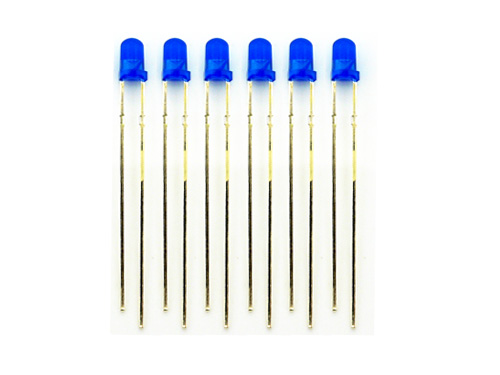
\includegraphics[width=5cm]{billeder/led.jpg}
\caption{3mm blue led}
\end{figure}
\item[] \textbf{Sensors} are some of the main components behind the Arduino success. They give the Arduino the ability to sense its surroundings. For instance the temperature of the room, whether the light is on of off, even advanced sensors like humidity, or gas sensor.
\begin{figure}[H]
\centering
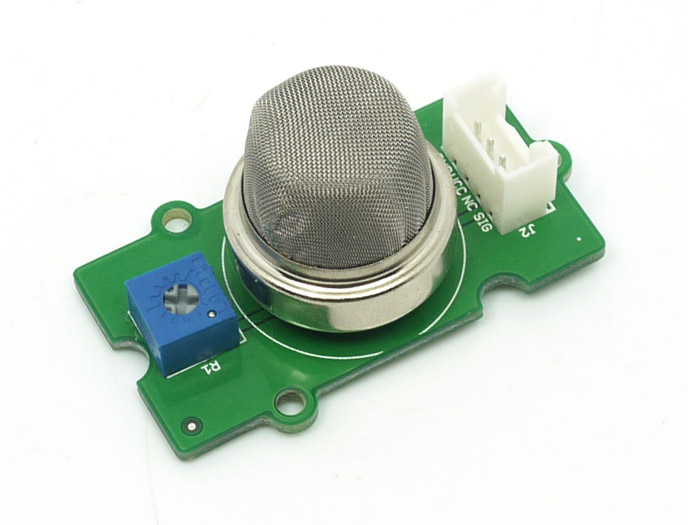
\includegraphics[width=5cm]{billeder/Sensor.jpg}
\caption{Gas sensor}
\end{figure}
\item[] \textbf{Motors} gives Arduino the ability to manipulate its surrounding, and act on the informations obtained from the sensors. There are two kind of motors, normal motors which can just be turned on/off. They are great for powering wheels or tracks. There are stepper motors, with these it is possible to control the exact amount of rotation. A more advanced version of the stepper motors are servo motors, with which more precise control is possible.
\begin{figure}[H]
\centering
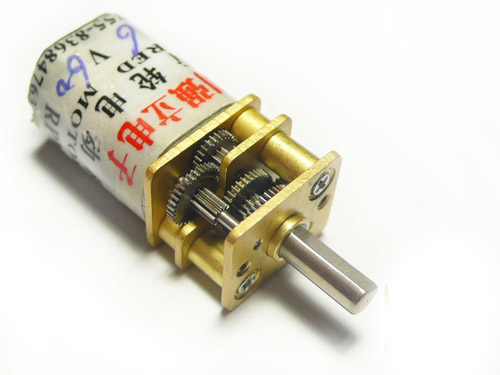
\includegraphics[width=5cm]{billeder/Motor.jpg}
\caption{Geared stepper motor}
\end{figure}
\item[] \textbf{Displays} are available in a wide range. Ranging from simple 2 line mono color LCD displays, all the way up to large OLED color and touch displays. 
\begin{figure}[H]
\centering
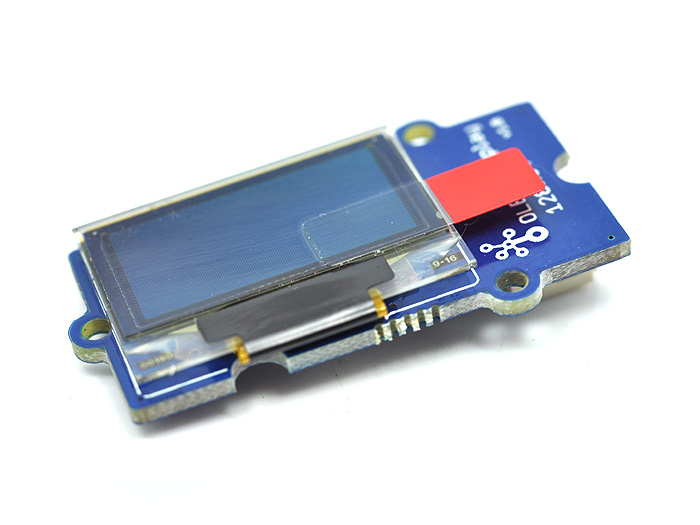
\includegraphics[width=5cm]{billeder/display.jpg}
\caption{OLED touch display}
\end{figure}
\item[] \textbf{Communication} components are easy to connect up on Arduino. This is allows it to communicate with other devices through either RF signals, Bluetooth, WiFi, cellular or just Ethernet connection.
\begin{figure}[H]
\centering
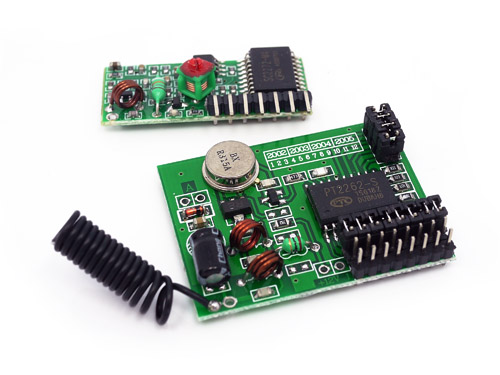
\includegraphics[width=5cm]{billeder/com.jpg}
\caption{RF transmitter and reciever}
\end{figure}
\item[] \textbf{Shields} are the components that makes the Arduino Platform great. They offer great  to the platform by allowing them to be plugged directly on to the Arduino. This makes it possible for anyone without any experience in electronics  to use them Shields are boards much like Arduino itself, but they offer all the capabilities of the components mentioned above.
\begin{figure}[H]
\centering
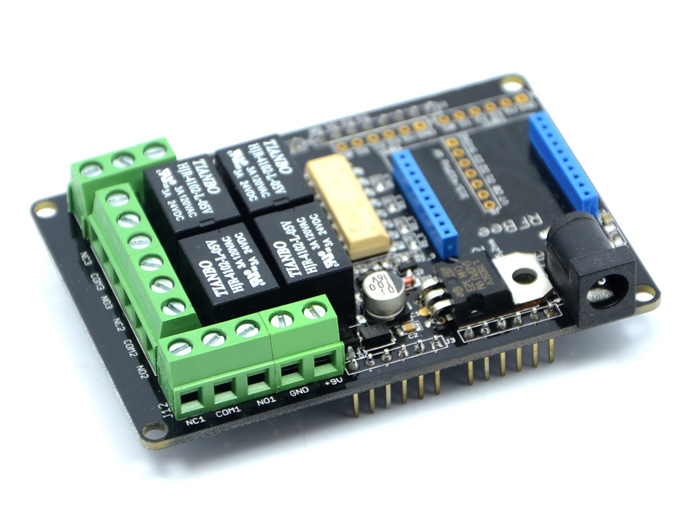
\includegraphics[width=5cm]{billeder/Shield.jpg}
\caption{Relay shield}
\end{figure}

\end{itemize}



\section{The purpose of the Arduino in this project}

In this project the arduino board will be used to execute the code, and show a type of output. The output will be in the form of a LCD Display and an LED light. 
The arduino in this project will also be able to get input through buttons and sensors. 
\fixme{Revise when we have the arduino!}

\part{Analysis} \label{chap:analysis}
\chapter{The compiler} \label{chap:the_compiler}
A compiler is a program which translates one language into another. When writing a program, the programmer uses a source language such as Java or C. A computer however only "understands" the language of binary code, the so called machine code. Binary code is in this case the target language reached by translating the source language into the target language, with the use of a compiler. Writing the program in binary code is however not optimal for the programmer as the alphabet of binary consists of 0's and 1's, and is hard to understand for human. So writing a program in a high level language such as Java or C and compiling it into machine code is easier for the programmer.
The goal of this project is to translate a high-level language to another high-level language - namely, from the source language to the Arduino language. The task of translating a programming language into another can be done using a compiler which is, basically, a translator. The compiler allows the programmer to avoid using the target language. The compiler is therefore responsible for always producing a correct representation of source language in the target language.

\section{The structure of a compiler} 
\label{sec:compiler}
Compiling a source language into a target language is not a one step process. The compiler goes through several steps in order to translate a program written in a source language into a program written in the target language. Some steps are necessary, and others are optional.

\begin{itemize}
	\item The first step performed by a compiler is the scanner, which prepares the source code for further treatment. This is done by running through the entire program one character at a time. Any unneeded code, such as the comments, is removed in this process. Every other part of the code is placed in groupings called tokens. These can for example be integers, identifiers and operators. Any user defined elements is furthermore put into a symbol tree, which is accessible throughout the process of compilation. If the user has defined, for example, that whenever the word ``POWER'' is written in the code of the program, it always refers to the number ``9001'', this would be put into the symbol tree. The result is that whenever ``POWER'' is found in the code, it will be replaced with ``9001''. After the source program has been run through, the output from the scanner is passed on to the parser.
	
	\item The second step is the parser, which analyses the syntax of the code received from the scanner. The parser checks if the syntax of the program is compatible to the syntax of the source language. If the written code is not proper according to the source language, it is not possible to be translated correctly. As an example, a C parser will return an error if the code states $a + b = c;$ rather than $c = a + b;$ this is because the syntax of the first expression is illegal in C. It is important to note that at this step it is unknown what the variables contain, which is where the type checker takes over.

	\item After the syntax has been verified, the third step is the type checker, which deals with the semantics of the source code. The type checker verifies that all operations performed in the code are legal with regard to the source language. In the previous example, $c = a + b;$ is syntactically correct. However what has not been specified is the content of a, b and c. If a and b are strings, while c is of the type int, the semantic is incorrect and will therefore return an error as the operation does not exist in the defined source language. If no errors occur, the parser will return an abstract syntax tree (AST) which also concludes the analysis of the source code. As seen in figure \ref{fig:ast_example} the AST shows the syntactic constructs. For example, an assignment requires a variable and an expression. 
	
	\begin{figure}[H]
	\centering
		\includegraphics{billeder/example_ast.png}
		\caption{AST example}
		\label{fig:ast_example}
\end{figure}
	
	

	\item At this point, the preparation of the source code is complete and the translation into the target language can be performed correctly. This is done by the translator. The translator translates the generated AST, from the parser, to an executable form. To translate the AST code generation visitors (CodeGenVisitor) are used, which visit the nodes in the AST. There are various different CodeGenVisitors to generate the right low-level language code. The output from the translator is the compiled product of the source code.
\end{itemize}

While this covers the direct compiling process, more optional steps can be used to enhance the compiling process for different purposes.\\

\begin{itemize}
\item An optimizer can be used to produce more effective code in the target language. While a piece of code can be optimal in the source language, the target language might have a more efficient formulation for describing the same action than the direct translation produces. The optimizer locates code which can be optimized and replaces the code with the more efficient model.

\end{itemize}
 %Introduction to a compiler
\chapter{Source language}\label{analysis:source-language}
In this project a new programming language, Basic Arduino Language (BAL), is proposed. The language is designed for the use of beginners in the field of programming and it is meant  to be an alternative for the already existing Arduino programming language.
The goal of the new language, the source language, is to make programming simpler and easier to understand compared to the existing Arduino programming language. The syntax is meant to be intuitive in that it can be read naturally, similar to the English language.

The source language is compiled to the Arduino language, rather than machine code. The source language is not a fully functioning programming language with advanced features. However, it is a simple language that can print out text and handle simple mathematics, such as adding, subtracting, multiplying numbers etc. along with handling boolean expressions built up from equalities and inequalities of numeric expressions.

The features for the source language are listed below:
\begin{itemize}
	\item It is readable, also by users that are not familiar with programming languages.
	\item It is easy to learn, and to be used for basic programming.
	\item It can be compiled to Arduino.
	\item The language is able to handle mathematics and boolean expressions.
\end{itemize} %Section about the new programming language.
\section{Language functions}
To get an overview and a basic representation of importance the language functions has been split into groupings called:
\begin{itemize}
\item \textbf{Could have}: features that would be nice to have, but are not of greater importance to accomplish for this project.

\item \textbf{Should have}: features that are important to the project but does not impair the core functionality of the project.

\item \textbf{Must have}: features that can not be left out in order to still have a functional language for the purpose of the project.
\end{itemize}

\textbf{Could haves:} \\

User input \\
While definitely a feature which is relevant for some purposes, the feature is not required in order to have a programming language able to use the features of Arduino. \\

Advanced mathematical operators \\
Mathematics can be solved without the use of integrated mathematics such as square root and modulus, but having the features is definitely convenient. \\

Loops (Other than while) \\
The ``while'' has all the functionality needed, but in some cases there are more intuitive ways to go around a problem. ``Foreach'' is a good example of this problem.\\

\textbf{Should haves:} \\

Initialization \\
There are different ways that initialization can work depending on the language as well as the type of the object. 

\textbf{Must haves:} \\

If-statement \\
The feature of choosing one path over another is so common to programming that it would make no sense to leave it out. One must be able to choose what to do based on something important to the program. \\

Boolean expressions \\
In relation to if-statements it makes little sense to leave out the ability to evaluate expressions to true or false. \\

Functions, parameters and return values \\
The ability to reuse code can reduce the cluttering of code significantly. While it may be possible to leave out functions, it will not make sense from a user-friendly perspective. Making use of parameters and return values removes the complexity of passing by reference. \\

Loop - While \\
Another very common task is to repeat the same task multiple times. Instead of having to create the code multiple times it is more user friendly to simple run the same piece of code, and is as such a must have. \\

Blocks (do/end signs) \\
Making it clear for the user where a block begins and ends helps reduce confusion. For example it might be hard to figure where a while loop ends if it has no ``end'' keyword or other recognizable sign. \\

Print \\
The ability to print out the results of a program is an easy way for the programmer to see the outcome. It is easy and user friendly. \\

Logical operators \\
Being able to select and group operators is important to perform decision making in programs. It would be very difficult to leave out of a general purpose language.\\

Simple mathematical operators \\
Leaving out mathematics removes a lot of functionality and heavily reduces the options of programming. \\

Type definitions \\
The user has to be capable of identifying what is being used. Without clearly defined types to use it can be very difficult for a beginner to understand how to program. \\

Imperative language \\
Choosing Imperative language means that the user will have to write code, that describes in exact details what steps has to be done and what step is the next one. Imperative language is supported by most of the mainstream object-oriented programming languages such as Java, C\#. \ref{Impr}

UTF-8 \\
The reason UTF-8 is a must have is because the typeset is very broad. This means the user does not have to worry about whether or not his special characters is acceptable characters, and does as such give the user the ability to code naturally. %Argumentation for inclusion of features
\section{The Arduino language}
The Arduino language is based on Wiring, which is an open source development platform, and therefore there are a lot of similarities between the two languages, but the Arduino team have added to it, improved the functions, and made it compatible with a wider range of chips. Both languages are implemented as versions of C/C++, and are using an IDE based on the processing IDE \cite{Wiring:thesis}\cite{Arduino:IDE}.\\

In table \ref{tabel:comparison}, the syntax of the two languages are almost identical, and it is only in the functions parameters, that there are any noticeable difference.\\ 
To help facilitate the compatibility with a wide range of AVR chips, the Arduino language makes great use of AVR Libc \cite{AVR:lib}, which is an open source C library that supplies the necessary functionality to make it possible to use the Atmel AVR micro controllers.\\

\begin{table}[H]
\centering
\begin{tabular}{cc}
Wiring 
& 
Arduino \\ 
\hline 
\begin{lstlisting}
int ledPin = 8;

void setup(){
  pinMode(ledPin, OUTPUT);
}
void loop(){
  digitalWrite(ledPin, HIGH);
  delay(1000);
  digitalWrite(ledPin, LOW);
  delay(1000);
}
\end{lstlisting}  
& 
\begin{lstlisting}
int led = 13;

void setup() {                
  pinMode(led, OUTPUT);     
}
void loop() {
  digitalWrite(led, HIGH);
  delay(1000);
  digitalWrite(led, LOW);
  delay(1000);
}
\end{lstlisting} 
\end{tabular} 
\caption{Code examples in both Wiring and Arduino to make a LED flash}
\label{tabel:comparison}
\end{table}
\todo{Kunne det ikk være brugbart at sætte et eksempel af C op ved siden af dem også?}


%\chapter{Compiler language}
The compiler is basically a program. This means that it is coded in a language and the choice of the programming language is a fundamental decision. Considering several programming languages, the one that was Java. With cross-platform capability\cite{java:requirements} and the fact that it has the features of object orientation\cite{java:object:orientation}. Furthermore Java has some strong similarities to the language C\#\cite{java:comparison}. Though C\# does not meet the requirements in terms of being cross-platform (It is not available for Mac users). \todo{Angiv kilde} %Choice of compiler language
%\input{Syntax and Semantics}
\chapter{Informal Specification}\label{analysis:informal-specification}
The purpose of this section is to outline what the programming language BAL, proposed in this project, contains.
\\The language created in this project is a simplification of the Arduino language. Its purpose is to simplify the process of writing programs for Arduino.   

\subsection{Data Types}
The language contains the following data types: \\ 
\begin{center}
\begin{tabular}{ l l l l}
int & float & string & boolean \\
\end{tabular}
\end{center}

The different data types can hold different ranges or types of values. The values are specified more below: 
\begin{itemize}
\item \textbf{Int} or integer can hold numbers between $-2^{15}$ and $2^{15}-1$. Integers do not include floating point numbers.
\item \textbf{Float} allows decimals as opposed to integers and have a range from $1.175494351e-38$ to $3.402823466e+384$.
%\item \textbf{Double} is the numeric type in the source language with the biggest range, which goes from $2.2250738585072014e-308$ to $1.7976931348623157e+308$.
\item \textbf{String} can hold any kind of number and/or character. 
%\item \textbf{Array} can consist of collections of elements, either values or variables. For instance it can hold numbers and/or string of characters. 
\item \textbf{Boolean} can either be [1] (true) or [0] (false). 
\end{itemize}

\subsection{Keywords}
The following words are reserved words in the programming language:\\ 
\begin{center}
\begin{tabular}{ l l l l l l}
if & else & elseif & do & end & function \\
while & return & true & false & int \\
float & string & void & loop & setup \\
\end{tabular}
\end{center}

\subsection{Variables}
The variables in the language can have any name represented by upper- and/or lower case English letters. In addition, the underscore sign ``\_ '' can also be used to make more complex variable-names. 

\subsection{Encapsulation}
The encapsulation in the language is defined by \textbf{do} and \textit{end}. \textit{do} opens the encapsulation, and \textbf{end} closes it.   

\subsection{Loops and Conditions}
The language contains a \textit{while-loop} with a condition check before the loop is executed. The language also contains an \textit{if do else} condition. Additionally, \textit{else if} can be used.   

\subsection{White-space and Commentary}
The compiler ignores the white-spaces as well as anything to the right-hand side of a comment, marked by ``//''. Additionally a block comment, marked by ``/* (comment here) */''.


%\subsection{Type conversion}
%\todo{Matti: Vi skal have defineret type conversion} % Informal specification
%
\section{The hardware structure of Arduino boards}
An Arduino is a small board, a single-board micro-controller.

The board were created to make a cheap way to control student-built interaction design projects. The board consist of open source hardware, which is designed around an 8-bit Atmel AVR micro-controller. The Arduino boards varies in sizes, but taking the Arduino Uno board as an example, then the board has a max width of 2.1'' and a length of 2.7''. 2.1'' is about 5,33cm and 2.7'' is about 6,86cm on the metric scale. 

The board provides some input and output possibilities, however this varies depending on the board, though most have 14 digital I/O and 6 analog inputs. The I/O functions is placed on top of the board, free accessible, and consists of 0.1'' female headers. Besides the I/O there is also Power connector, which is almost all cases will require 5 volt DC. There is an USB connection on the board, so that processing data to the micro-controller is possible, though it is shown as a virtual com-port on the connected computer. However on older boards, instead of the USB connection, a RS232 were used for serial communication. 

On the board there is an LED diode which is connected to the digital pin 13. When this diode is set to ``HIGH'' it will be turned on, and if its value is ``LOW'' it is off. Besides the LED diode there is also a reset button. If this button is pressed the micro-controller is reset. 

The Arduino board gain extra features through shields. Shields is a ``board'', or rather an expansion board, which is plugged onto the Arduino board. These can provide the Arduino board with the possibilities to control for example motors, sensors and LCD displays. This increases the many possibilities there is with an Arduino board. 

kilder:\todo{Jonas: ZAT!! DET ER FOR DOVENT AT SMIDE KILDER HER!}
\todo{Jonas: Sectionen bør nok hedde ``The Arduino board''. Og et billede ville ikke gøre skade.}

http://en.wikipedia.org/wiki/Arduino
http://en.wikipedia.org/wiki/File:UnoConnections.jpg
http://arduino.cc/en/Main/ArduinoBoardUno
 %Text about the Arduino hardware
%\chapter{Arduino}\label{analysis:arduino}
Arduino was created by the Interaction Design Institute Ivrea (Italy), by Massimo Banzi and David Cuartielles. They were looking for an easy and cheap way for students, who study design, to integrate micro controllers into their projects\cite{arduino:hist}. Both the board and the programming language was based on the works of Hernando Barragán, one of Massimo Banzi master thesis students \cite{Wiring:thesis}.

In this project Arduino board is used to execute the code, and show a type of output. The output will be in the form of a LCD Display. 

\section{The Hardware Components}
Arduino is a single-board micro-controller, see figure \ref{fig:Arduino_uno}.
A board consists of open source hardware, which is designed around an 8-bit Atmel AVR micro-controller. Arduino boards varies in sizes. Arduino Uno board for example, has a max width of 2.1'' (5,33cm) and a length of 2.7'' (6,86cm).  \\

\par
\raisebox{-.5\height}{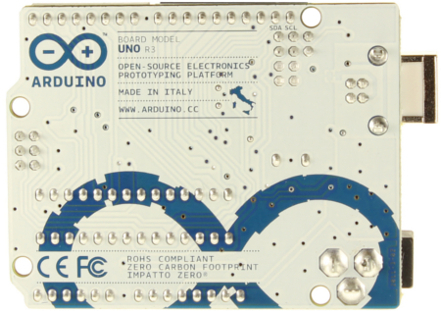
\includegraphics[width=6.5cm]{billeder/ArduinoUno_R3_Back_450px.jpg}}
\hfill
\raisebox{-.5\height}{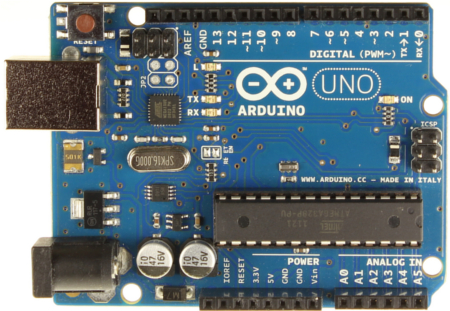
\includegraphics[width=6.5cm]{billeder/ArduinoUno_R3_Front_450px.jpg}}
\begin{figure}[H]
\caption{Picture of back- and fronside of the Arduino Uno board \cite{Arduino:board_pics}}
\label{fig:Arduino_uno}
\end{figure}
\par

\par
\raisebox{-.5\height}{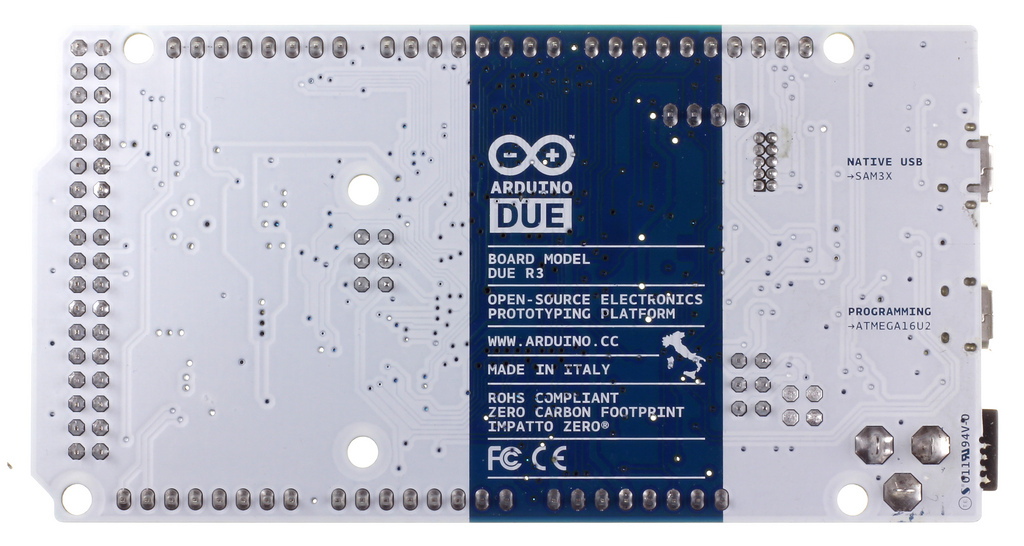
\includegraphics[width=6.5cm]{billeder/ArduinoDue_2.jpg}}
\hfill
\raisebox{-.5\height}{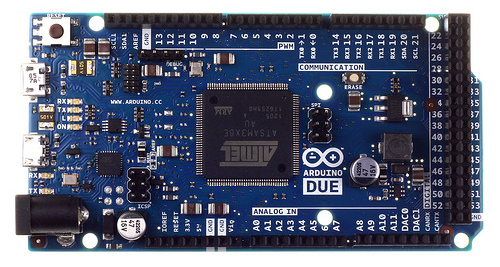
\includegraphics[width=6.5cm]{billeder/ArduinoDue_1.jpg}}
\begin{figure}[H]
\caption{Picture of back- and fronside of the Arduino Duo board \cite{Arduino:board_pics}}
\label{fig:Arduino_duo}
\end{figure}
\par

\subsection*{Specifications}
The board provides some input and output possibilities. The Arduino Uno, figure \ref{fig:Arduino_uno}, has 14 digital I/O and 6 analog inputs, where as the Arduino Due, figure \ref{fig:Arduino_duo}, has 54 digital, and 12 analog pins. The I/O functions are placed on top of the board, and are freely accessible, and consist of 0.1'' female headers. Besides the I/O there is also a Power connector, which almost in all cases require 5 volt DC. There is an USB connection on the board, so that processing data to the micro-controller is possible, though it is shown as a virtual com-port on the connected computer. However, on older boards, instead of the USB connection, a RS232 were used for serial communication. 

\begin{figure}[H]
\centering
\begin{tabular}{|c|c|}
\hline 
Microcontroller & ATmega328 \\ 
\hline 
Operating Voltage & 5V \\ 
\hline 
Input Voltage (recommended)	 & 7-12V \\ 
\hline 
Input Voltage (limits) & 6-20V \\ 
\hline 
Digital I/O Pins & 14 (of which 6 provide PWM output) \\ 
\hline 
Analog Input Pins & 6 \\ 
\hline 
DC Current per I/O Pin & 40 mA \\ 
\hline 
DC Current for 3.3V Pin & 50 mA \\ 
\hline 
Flash Memory & 32 KB (ATmega328) of which 0.5 KB used by bootloader \\ 
\hline 
SRAM & 2 KB (ATmega328) \\ 
\hline 
EEPROM & 1 KB (ATmega328) \\ 
\hline 
Clock Speed & 16 MHz \\ 
\hline 
\end{tabular} 
\caption{Hardware specifications for the Arduino Uno}
\end{figure}

On the board there is a LED, which is connected to the digital pin 13. When this diode is set to ``HIGH'' it will be turned on, and if its value is ``LOW'' it turns off. Besides the LED, there is also a reset button. If the button is pressed the micro-controller is reset. 

The specifications, which are important to take into consideration in regard to designing a programming language aimed at the Arduino platform, is the flash memory, the main memory(SRAM) and the CPU speed. The most limiting factor to take into consideration is the amount of RAM, the larger and more complex the data structures are, the bigger the risk of running out of memory while executing a program. Although this is not limited to developing for the Arduino platform, it is certainly a larger factor, then when developing for desktop computers.
Another factor that need attention is the flash memory, meaning the pace available for the program, the smallest example code for the Arduino, the Blink example listings \ref{lst:blink}, only uses 1084 bytes, which is approximately $3.3 \%$ of the total memory available. 

\begin{table}[h!]\scriptsize
\centering
\begin{tabular}{cc} 
\begin{minipage}{6cm}
{\begin{lstlisting}[caption=Arduino,frame=none,resetmargins=true,label={lst:blink}]
int led = 13;
void setup() {                
  pinMode(led, OUTPUT);     
}

void loop() {
  digitalWrite(led, HIGH);   
  delay(1000);    
  digitalWrite(led, LOW);  
  delay(1000);
}
\end{lstlisting}}
\end{minipage}
  & 
\begin{minipage}{10cm}
{\begin{lstlisting}[caption=C\#,frame=none,resetmargins=true,label={lst:C_hello}]
namespace hello
{
  class Program
  {
    static void Main(string[] args)
    {
       System.Console.WriteLine("Hello, World!");
       System.Console.ReadKey();
    }
  }
}
\end{lstlisting}}
  \end{minipage}
 \\ 
 \end{tabular} 
 \caption{Comparison between a simple Arduino and C\# example}
 \end{table} 

If a language has a lot of complex features, it will quickly run out of space. For instance with more complex languages like C\#, a simple hello world, listings \ref{lst:C_hello}, program uses 5120 bytes, and they can quickly run in the hundreds or thousands of kilobytes. This is even more important to remember, when one takes into account, that there are many different Arduino configurations, and the language have to function on all of them. The Arduino Nano for instance, only has 16 KB of memory, and there are Arduino clones by other manufactures with even less.



\subsection*{Components}
What makes Arduino such a good platform for beginners to learn to program on, is because it is really easy to connect a wide variety of components to it, making it possible for the Arduino to interact with the real world.

\begin{itemize}
\item[] \textbf{LED's} come in all size, shapes and colors, ranging from small pin size single color LED's, to large multi color LED displays.
\begin{figure}[H]
\centering
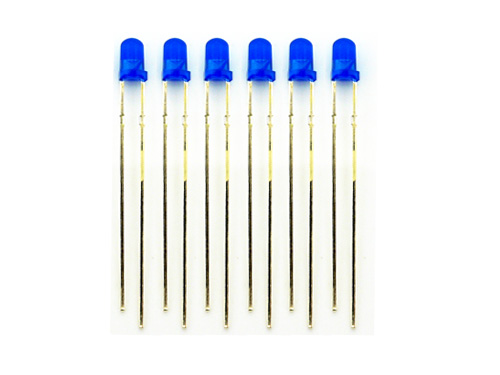
\includegraphics[width=5cm]{billeder/led.jpg}
\caption{3mm blue led}
\end{figure}
\item[] \textbf{Sensors} are some of the main components behind the Arduino success. They give the Arduino the ability to sense its surroundings. For instance the temperature of the room, whether the light is on of off, even advanced sensors like humidity, or gas sensor.
\begin{figure}[H]
\centering
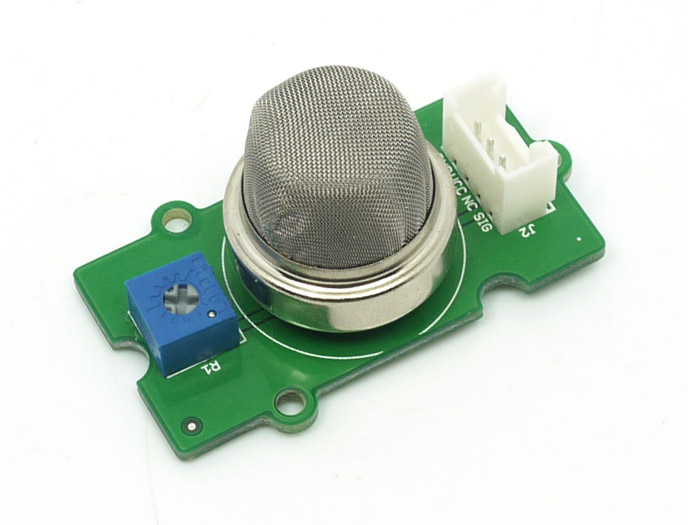
\includegraphics[width=5cm]{billeder/Sensor.jpg}
\caption{Gas sensor}
\end{figure}
\item[] \textbf{Motors} gives Arduino the ability to manipulate its surrounding, and act on the informations obtained from the sensors. There are two kind of motors, normal motors which can just be turned on/off. They are great for powering wheels or tracks. There are stepper motors, with these it is possible to control the exact amount of rotation. A more advanced version of the stepper motors are servo motors, with which more precise control is possible.
\begin{figure}[H]
\centering
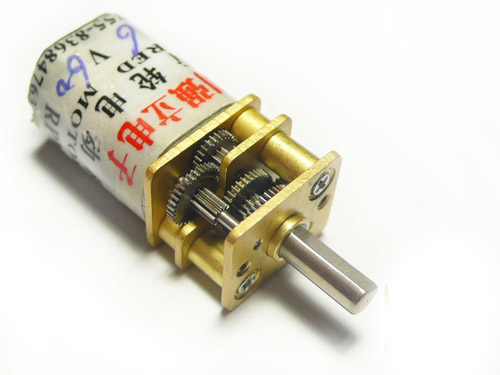
\includegraphics[width=5cm]{billeder/Motor.jpg}
\caption{Geared stepper motor}
\end{figure}
\item[] \textbf{Displays} are available in a wide range. Ranging from simple 2 line mono color LCD displays, all the way up to large OLED color and touch displays. 
\begin{figure}[H]
\centering
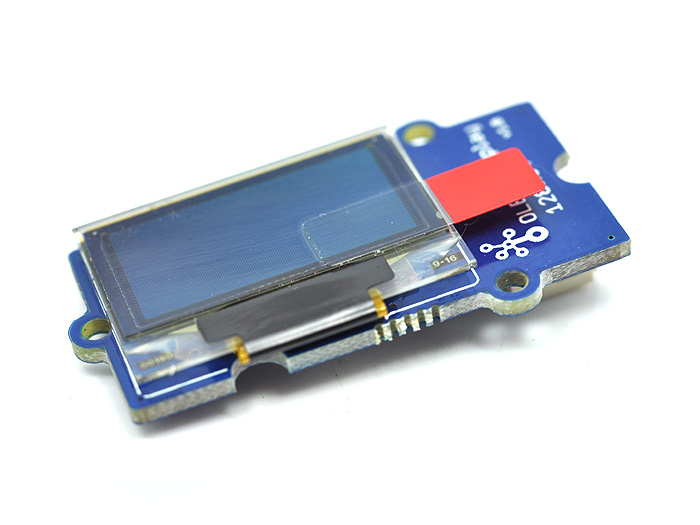
\includegraphics[width=5cm]{billeder/display.jpg}
\caption{OLED touch display}
\end{figure}
\item[] \textbf{Communication} components are easy to connect up on Arduino. This is allows it to communicate with other devices through either RF signals, Bluetooth, WiFi, cellular or just Ethernet connection.
\begin{figure}[H]
\centering
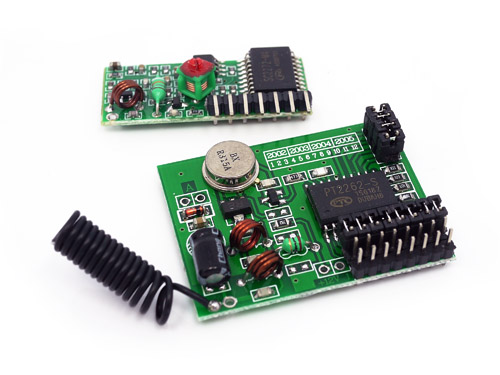
\includegraphics[width=5cm]{billeder/com.jpg}
\caption{RF transmitter and reciever}
\end{figure}
\item[] \textbf{Shields} are the components that makes the Arduino Platform great. They offer great  to the platform by allowing them to be plugged directly on to the Arduino. This makes it possible for anyone without any experience in electronics  to use them Shields are boards much like Arduino itself, but they offer all the capabilities of the components mentioned above.
\begin{figure}[H]
\centering
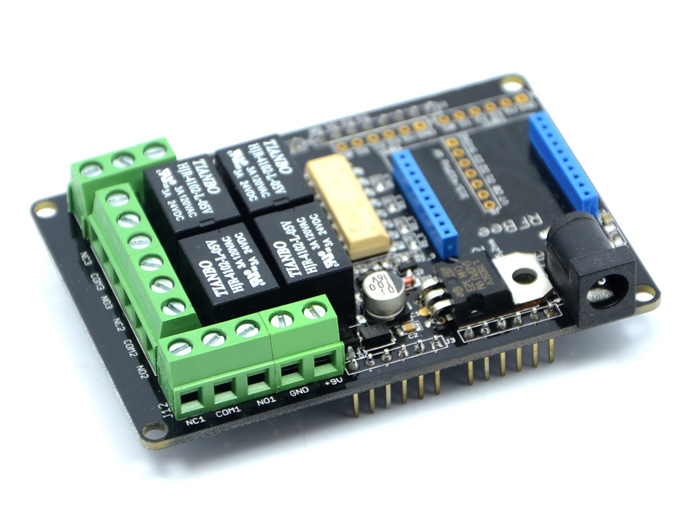
\includegraphics[width=5cm]{billeder/Shield.jpg}
\caption{Relay shield}
\end{figure}

\end{itemize}


 % Section about the Arduino language
%\section{The purpose of the Arduino in this project}

In this project the arduino board will be used to execute the code, and show a type of output. The output will be in the form of a LCD Display and an LED light. 
The arduino in this project will also be able to get input through buttons and sensors. 
\fixme{Revise when we have the arduino!}
\chapter{Syntax and Semantics}\label{analysis:syntax-and-semantics}
In this section the syntax and semantics of the source language is described. It contains a definition in the form of Extended Backus-Naur Form and the transition rules of the language

\section{Syntax}
When describing a programming language, the syntax of the language is given by the set of rules which defines the words (finite sequences of characters) that can be used for writing a program in that language. The syntax of the language is described using \textit{Backus-Naur Form} (BNF) which provides the context free grammar of the language.
In this report an extended version of BNF, \textit{Extended Backus-Naur Form} (EBNF), is used. The advantage of using EBNF is to describe the set of rules in a more compact form, and the ability to describe regular expressions in the context free grammar. EBNF does not enhance the descriptive power of BNF, it only increases the readability and the write-ability.

\section{Syntax definition}\label{sec:anlysis:syntax-definition}
Following is the syntax definition written in EBNF which shows the seven syntactic categories followed by the defined rules. As an example of how to read these rules, let $a$ be an arithmetic expression. By looking at the rule for $a$, this expression could for example be $a_1 + a_2$ meaning it is expanded to be one arithmetic expression consisting in the addition of two other arithmetic expressions. These two expressions could then again be anything within the rules for $a$, for example the numerals 5 and 7. There are no rules for expanding a numeral, and as such the expression $a$ can be evaluated no further.
\begin{lstlisting}[mathescape, captionpos=b, caption=Syntax formation rules, label=lst:syntax-formation]
$n$ $\in$ Num - Numerals
$x$ $\in$ Var - Variables
$a$ $\in$ Aexp - Arithmetic expressions
$b$ $\in$ Bexp - Boolean expressions
$S$ $\in$ Stm - Statements
$Dv \in$ DecV - Variable declarations
$S_b$ $\in$ Substatement

$a$ ::= $n$ | $x$ | $a_1 + a_2$ | $a_1 - a_2$ | $a_1 * a_2$ | $a_1 / a_2$ | sqrt($a$) | $a_1$^$a_2$ | $a_1$ % $a_2$ | ($a$)

$b$ ::= "$a_1$ equals $a_2$" | "$a_1 > a_2$" | "$a_1 < a_2$" | "$a_1 <= a_2$" | "$a_1 >= a_2$" | "$a_1$ notequals $a_2$" | not$b$ | $b_1$ and $b_2$ | $b_1$ or $b_2$ | ($b$)

$S$ ::= $Dv$ | if $b$ do $S$ end $S_b$ | while $b$ do $S$ end | $S_1 ; S_2$

$S_b$ ::= {elseif $b$ do $S$ end} | else do $S$ end

$Dv$ ::= $x$ = $a$; Dv
\end{lstlisting}

\subsection{Numerals}
In BAL there are two numeral systems called \textit{integers} and \textit{floats}. These types are needed to represent integers (for example -17, -239586, 0, 237, 9001). and decimal numbers (such as -12.3456, -30.009, 90.01 and 990.1259). Float is used for decimal numbers. The numeral systems are however finite as the numerals can not exceed the size allocated to each float, integer and double. As such the limitations are:
\begin{itemize}
\item Integers: From $-2^{15}$ to $2^{15}-1$
\item Floats: From $3.4E-38$ to $3.4E+38$
\end{itemize}

\subsection{Variables}
A variable in the language ranges over text strings, arithmetic expressions, boolean expression, and numerals

%\subsection{Metavariables}
%\todo{Distinction between variables and metavariables is needed, what is meta variables?}

\subsection{Arithmetic expressions}
The source language features arithmetic expressions. The rules listed in listing \ref{lst:syntax-formation} states that well-formed arithmetic expressions in the source language can consist of:
\begin{itemize}
	\item x - Variable
	\item n - Numeral
	\item Addition "$a_1 + a_2$" - Addition between two numbers.
	\item Subtraction "$a_1 - a_2$" - Subtraction between two numbers.
	\item Multiplication "$a_1 * a_2$" - Multiplication between two numbers.
	\item Division "$a_1 / a_2$" - Division between two numbers.
	\item Square root "sqrt($a$)" - Finds the square root of a number.
	\item Power "$a_1$\texttt{\^{}}$a_2$" - Allows a number to be exponentiated by another number.
	\item Modulus "$a_1$ \% $a_2$" - Allows modulus to be used, which gives the opportunity to find the remainder of a division between two arithmetic expressions.
	\item Parenthesis "($a$)" - Specifies that an expression can be surrounded by parenthesis.
\end{itemize}

\subsection{Boolean expressions}
The source language supports boolean expressions, which evaluate to \textit{true} or \textit{false}.
\begin{itemize}
	\item Equals to ($a_1$ equals $a_2$) - $equals$ allows the programmer to equate two expressions, which will evaluates to \textit{true} if their evaluations match; if not it evaluates to \textit{false}.
	\item Greater than ($a_1 > a_2$) - ``$>$'' checks if one value is greater than another value. If $a_1$ is greater than $a_2$ it evaluates to \textit{true}, else it evaluates to \textit{false}.
	\item Less than ($a_1 < a_2$) - ``$<$'' checks if the value of the first expression is lesser than the value of the second one. If $a_1$ is less than $a_2$ it evaluates to \textit{true}, else \textit{false}.
	\item Greater than or equal to ($a_1 >= a_2$) - ``$>=$'' checks if one value is greater then or equals another value. If $a_1$ is greater then or equals $a_2$ it evaluates to \textit{true}, and it evaluates to \textit{false} otherwise.
	\item Less than or equal to ($a_1 <= a_2$) - ``$<=$'' checks if one value is less then or equals another value. If $a_1$ is less then or equals $a_2$ it evaluates to \textit{true}, and it evaluates to \textit{false} otherwise.
	\item Different from ($a_1$ notequals $a_2$) - ``$notequals$'' checks if two values are different. If $a_1$ is different from $a_2$ it evaluates \textit{true}, and it evaluates to \textit{false} otherwise. 
	\item Negation (not$b$) - ``$not$'' if $b$ is true it evaluates to false. If $b$ is \textit{false} it evaluates \textit{true}.
	\item Conjunction ($b_1$ and $b_2$) - ``$and$'' check if two boolean values are both \textit{true}. If both $b_1$ and $b_2$ are \textit{true} it evaluates \textit{true}, and it evaluates to \textit{false} otherwise. 
	\item Disjunction ($b_1$ or $b_2$) - ``$or$'' checks if one of the boolean values are \textit{true}. If either $b_1$ or $b_2$ are \textit{true} it evaluates \textit{true}, and it evaluates to \textit{false} otherwise.
	\item Parenthesis (($b$)) - Allows the boolean expressions to be insulated in parenthesis. The parenthesis will then evaluate to \textit{true} or \textit{false}.
\end{itemize}
\subsection{Statements}

$S$ ::= Dv | if $b$ do $S$ end $S_b$ | while $b$ do $S$ end | $S_1 ; S_2$

\begin{itemize}
	\item Variable declaration - The rule states that a variable declaration is composed by variable name on the lefthand side of the assignment character ``='', and then the value (of the arithmetic expression) on the righthand side is thereby assigned to the left side. The ``;'' character closes the variable declaration.
	\item If-statement -  A conditional expression involving one boolean expression and two statements, or a statement and a substatement. If the boolean expression evaluates to true, the first statement is executed. If the boolean condition evaluates to false, then the program executes the second statement or the substatement.

	\item While loop - It involves a boolean expression and the while loop will run if the boolean expression evaluates to true. As long as the boolean expression is true, the statements inside the loop is repeatedly executed. When the boolean expression evaluates to false, the loop is exited.
	\item Sequential Composition - To make programs execute statements sequentially in the source language.
\end{itemize}

\subsubsection{Substatements}

$S_b$ ::= {elseif $b$ do $S$ end} | else do $S$ end

\begin{itemize}
	\item Elseif - If an if-statement is executed the source language allows to follow up using an elseif statement. In the case an if-statement is not present, an elseif is not allowed to be used. Elseif follow the same rules as if-statements, and just like if-statements it has a boolean expression, which if it is true the statement is executed. If the boolean expression is evaluated to false, the program executes the second statement or the substatement.
	\item Else - If the boolean expression in an if-statement evaluates to false, an else statement can be reached which will execute the other statement. An if-statement is required to be able to use the else-statement.
\end{itemize}


%\section{Syntax}
%When describing a programming language the syntax of the language is given by the set of rules which defines the words (finite sequences of characters) that can be used for writing a program in that language. The syntax of the language is described using Backus-Naur Form (BNF) which provides the context free grammar of the language.
%In this report an extended version of BNF, Extended Backus-Naur Form (EBNF), is used. The advantage of using EBNF is to describe the set of rules in a more compact form, and the ability to describe regular expressions in the context free grammar. EBNF does not enhance the descriptive power of BNF, it only increases the readability and the write-ability.

%\subsection{Program}
% \begin{lstlisting}[captionpos=b, caption{EBNF of how a program needs to be structured.}]
% <program> -> void setup() begin <statement_list> end void loop() begin <statement_list> end
% <statement_list> -> (<statement> | <statement> ; <statement_list>
% \end{lstlisting}

% \subsection{IF-statement}
% The following EBNF describes how IF-statements can be used in the source language. It describes that the if-statement can be used in one of the three different ways:
% \begin{itemize}
% 	\item if(EXPRESSION) then STATEMENT end
% 	\item if(EXPRESSION) then STATEMENT elseif STATEMENT else STATEMENT end. The elseif statement can be used an infinite amount of times.
% 	\item If(EXPRESSION) then STATEMENT else STATEMENT end
% \end{itemize}
% \begin{lstlisting}[captionpos=b, caption={EBNF of the IF-statement in the source language}]
% <if_statement> -> if(<expression>) then <statement> [{elseif <statement>} else <statement> | else <statement>] end
% \end{lstlisting}


% \subsection{While loop}
% The following EBNF describes how the while loop is allowed to be used in the source language. Note that only a while loop is described, because no other loops than the while loop is part of the source language.
% \begin{lstlisting}[mathescape, captionpos=b, caption={EBNF of a while loop.}]
% <while_stmt> -> while (<expression>) do <statement> end
% \end{lstlisting}

% \subsection{Function}
% \begin{lstlisting}[mathescape, captionpos=b, caption={EBNF of a function.}]
% <function> -> function (<expression>) do <statement> end
% \end{lstlisting}

% \subsection{Assign}
% \begin{lstlisting}[mathescape, captionpos=b, caption{EBNF of how assignment work.}]
% <assign> -> <variable> = <expression>;
% \end{lstlisting}

% \subsection{Variables}
% \begin{lstlisting}[mathescape, captionpos=b, caption{EBNF of how a variable can be declared.}]
% <variable> -> (<arithmetic expression> | $\lambda$);
% \end{lstlisting}

% \subsection{Expression}
% \begin{lstlisting}[mathescape, captionpos=b, caption{EBNF of expressions.}]
% <arithmetic expression> -> <variable> (+ | - | *) <variable>;
% \end{lstlisting}

\section{Semantics} \label{sec:semantics}
The semantics of a language is the description of what happens when a program is executed.

Seen in table \ref{tab:semantics_aritmethic}, \ref{tab:semantics_boolean} and \ref{tab:semantics_statements} are the exact descriptions of the possible operations in our language. \ref{tab:semantics_aritmethic} describes all arithmetic actions - the more obvious ones are addition, subtraction, multiplication and division (PLUS, MINUS, MULT, DIV) which all look near identical: A statement, s, with two expressions, $v_{1}$ and $v_{2}$ which both are arithmetic as seen by $\rightarrow_{a}$ can be added, subtracted, multiplied or divided with each other. This results in $v$ which again is arithmetic. Furthermore $v$ is the product of the operator used on $v_{1}$ and $v_{2}$. Both modulus and power (MOD, POW) are identical to these operations in procedure. \\
SQRT is a simple rule to allow any arithmetic expression, $v_{1}$ to be squared, where $v$ obviously is $\sqrt{v_{1}}$. \\
The PARENT rule simply states that any arithmetic expression can be parenthesized, allowing chained arithmetic calculations to be performed in the correct order. VAR describes that in a state $s$ a value $v$ be assigned to a variable $x$ allowing variable declaration. NUM allows within a statement $S$ to get the numerical value of a variable $v$ \\

The table \ref{tab:semantics_boolean} holds the rules of boolean operations. Once again a lot of operations look near identical, namely EQUAL1, EQUAL2, NOTEQUAL1, NOTEQUAL2, GREATER1, GREATER2, LESSER1, LESSER2, LEQ1, LEQ2, GEQ1 and GEQ2. The common factor is that these are all comparison expressions, respectively checks for equality, greater than, less than, less or equal to and greater or equal to. Having a $v_{1}$ and $v_{2}$ which are both arithmetic as seen by $\rightarrow_{a}$, we use a boolean evaluation to conclude whether comparison is true (tt) or false (ff). \\
The NOT1, NOT2, AND1, AND2, OR1 and OR2 expressions are similar as well. Arithmetic expressions are tested with some criteria and evaluated to true or false. In the case of NOT1 where the evaluation is true, the evaluation of NOT1 is obviously false as it is not "not", with NOT2 being the opposite case. AND1, AND2, OR1 and OR2 follow same principles. In AND1 and AND2, two expressions need to be true if the entire expression is to be true, while OR1 and OR2 just needs one of two expressions. \\
As with the PARENT rule in table \ref{tab:semantics_aritmethic} any boolean expression can be parenthesized as well as seen in this PARENT rule. \\ \todo{The therminology should be corrected here.}

The table of statement semantics, \ref{tab:semantics_statements} holds rules affecting statements in any way. \\
ASS describes that with a given state and expression ($a, s$), a variable $x$ can be assigned a value $v$. The SKIP rule states that within a state $s$, a skip can occur, leading to a state $s$. COMP allows compositional statements meaning that a series of statements can occur. IFTRUE and IFFALSE allows choosing an appropriate substatement based on some boolean expression within a statement. \\ \todo{Morten: Missing WHILETRUE and WHILEFALSE. Help please.}

\begin{table}[h]
	\begin{tabular}{|l|l|l|}
	\hline
	\emph{Name}			& \emph{Rule}																															& \emph{Notes} \\ \hline
			~			&															~																			& ~ \\
	$[PLUS_{BSS}]$		& $s~\vdash~a_{1}~\rightarrow_{a}~v_{1}~~ s~\vdash~a_{2}~\rightarrow_{a}~v_{2} \over s~\vdash~a_{1}~+~a_{2}~\rightarrow_{a}~v$ 			& where $v = v_{1}+v_{2}$ \\
			~			&															~																			& ~ \\
	$[MINUS_{BSS}]$		& $s~\vdash~a_{1}~\rightarrow_{a}~v_{1}~~s \vdash a_{2}~\rightarrow_{a}~v_{2} \over s~\vdash~a_{1}~-~a_{2}~\rightarrow_{a}~v$ 			& where $v = v_{1}-v_{2}$ \\
			~			&															~																			& ~ \\
	$[MULT_{BSS}]$		& $s~\vdash~a_{1}~\rightarrow_{a}~v_{1}~~s~\vdash a_{2}~\rightarrow_{a}~v_{2} \over s~\vdash~a_{1}~*~a_{2}~\rightarrow_{a}~v$ 			& where $v = v_{1}*v_{2}$ \\
			~			&															~																			& ~ \\
	$[DIV_{BSS}]$		& $s~\vdash a_{1}~\rightarrow_{a}~v_{1}~~s ~\vdash a_{2}~\rightarrow_{a}~v_{2} \over s~\vdash~{a_{1}}~/~{a_{2}}~\rightarrow_{a}~v$ 		& where $v = \frac{v_{1}}{v_{2}}$ and $v_2 \neq 0$\\
			~			&																																		& ~ \\
	$[MOD_{BSS}]$		& $s~\vdash a_{1}~\rightarrow_{a}~v_{1}~~s~\vdash~a_{2}~\rightarrow_{a}~v_{2} \over s~\vdash~a_{1}~\%~a_{2}~\rightarrow_{a}~v$			& where $v = v_{1}\%v_{2}$ \\
			~			&															~																			& ~ \\
	$[POW_{BSS}]$		& $s~\vdash~a_{1}~\rightarrow_{a}~v_{1}~~s~\vdash~a_{2}~
	\rightarrow_{a}~v_{2} \over~s~\vdash~a_{1}~\texttt{\^{}}~a_{2}~\rightarrow_{a}~v$	& where $v = v_{1}\texttt{\^{}}v_{2}$ \\
			~			&															~																			& ~ \\
	$[SQRT_{BSS}]$		& $s~\vdash~a_{1}~\rightarrow_{a}~v_{1} \over s~\vdash~sqrt(a_{1})~\rightarrow_{a}~v_{1}$												& where $v = \sqrt{v_{1}}$ and $v_1 >= 0$ \\
			~			&															~																			& ~ \\
	$[PARENT_{BSS}]$	& $s~\vdash a_{1}~\rightarrow_{a}~v_{1} \over s~\vdash~(a_{1})~\rightarrow_{a}~v_{1}$													& ~ \\
			~			&															~																			& ~ \\
	$[NUM_{BSS}]$		& $s~\vdash~n~\rightarrow_{a}~v~ if ~\mathcal{N}\llbracket n \rrbracket~=~v$															& ~ \\
			~			&															~																			& ~ \\
	$[VAR_{BSS}]$		& $s~\vdash~x~\rightarrow_{a}~v~if~sx~=~v$														   									& ~ \\
			~			&															~																			& ~ \\
	\hline
	\end{tabular}
	\label{tab:semantics_aritmethic}
	\caption{The semantics of arithmetic operations}
\end{table}

\begin{table}[h]
	\begin{tabular}{|l|l|l|}
	\hline
	\emph{Name}			& \emph{Rule}																															& \emph{Notes} \\ \hline
			~			&															~																			& ~ \\
	$[NOT1_{BSS}]$		& $s~\vdash~b_{1}~\rightarrow_{b}~tt \over s~\vdash~not~b_{1}~\rightarrow_{b}~ff$														& ~ \\
			~			&															~																			& ~ \\
	$[NOT2_{BSS}]$		& $s~\vdash~b_{1}~\rightarrow_{b}~ff \over s~\vdash~not~b_{1}~\rightarrow_{b}~tt$														& ~ \\
			~			&															~																			& ~ \\
	$[EQUAL1_{BSS}]$	& $s~\vdash~a_{1}~\rightarrow_{a}~v_{1}~~s~\vdash a_{2}~\rightarrow_{a}~v_{2} \over s~\vdash~a_{1}~equals~a_{2}~\rightarrow_{b}~tt$		& if $v_{1} = v_{2}$ \\
			~			&															~																			& ~ \\
	$[EQUAL2_{BSS}]$	& $s~\vdash~a_{1}~\rightarrow_{a}~v_{1}~~s~\vdash~a_{2}~
	\rightarrow_{a}~v_{2} \over s~\vdash~a_{1}~equals~a_{2}~\rightarrow_{b}~ff$		& if $v_{1} \ne v_{2}$ \\
			~			&															~																			& ~ \\
	$[NOTEQUAL1_{BSS}]$	& $s~\vdash~a_{1}~\rightarrow_{a}~v_{1}~~s~\vdash~a_{2}~
	\rightarrow_{a}~v_{2} \over s~\vdash~a_{1}~notequals~a_{2}~\rightarrow_{b}~tt$	& if $v_{1}\ne v_{2}$ \\
			~			&															~																			& ~ \\
	$[NOTEQUAL2_{BSS}]$	& $s~\vdash~a_{1}~\rightarrow_{a}~v_{1}~~s~
	\vdash~a_{2}~\rightarrow_{a}~v_{2} \over s~\vdash~a_{1}~notequals~a_{2}~\rightarrow_{b}~ff$	& if $v_{1} = v_{2}$ \\
			~			&															~																			& ~ \\
	$[GREATER1_{BSS}]$	& $s~\vdash~a_{1}~\rightarrow_{a}~v_{1}~~s~
	\vdash~a_{2}~\rightarrow_{a}~v_{2} \over s~\vdash~a_{1}~<~a_{2}~\rightarrow_{b}~tt$			& if $v_{1} < v_{2}$ \\
			~			&															~																			& ~ \\
	$[GREATER2_{BSS}]$	& $s~\vdash~a_{1}~\rightarrow_{a}~v_{1}~~s~
	\vdash~a_{2}~\rightarrow_{a}~v_{2} \over s~\vdash~a_{1}~<~a_{2}~\rightarrow_{b}~ff$			& if $v_{1} \not< v_{2}$ \\
			~			&															~																			& ~ \\
	$[LESSER1_{BSS}]$	& $s~\vdash~a_{1}~\rightarrow_{a}~v_{1}~~s~\vdash~a_{2}~
	\rightarrow_{a}~v_{2} \over s~\vdash~a_{1}~>~a_{2}~\rightarrow_{b}~tt$			& if $v_{1} > v_{2}$ \\
			~			&															~																			& ~ \\
	$[LESSER2_{BSS}]$	& $s~\vdash~a_{1}~\rightarrow_{a}~v_{1}~~s~\vdash a_{2}~\rightarrow_{a}~v_{2} \over s~\vdash~a_{1}~>~a_{2}~\rightarrow_{b}~ff$			& if $v_{1} \not> v_{2}$ \\
			~			&															~																			& ~ \\
	$[LEQ1_{BSS}]$		& $s~\vdash~a_{1}~\rightarrow_{a}~v_{1}~~s~\vdash~a_{2}~
	\rightarrow_{a}~v_{2} \over s~\vdash~a_{1}~>=~a_{2}~\rightarrow_{b}~tt$			& if $v_{1} \leq v_{2}$ \\
			~			&															~																			& ~ \\
	$[LEQ2_{BSS}]$		& $s~\vdash~a_{1}~\rightarrow_{a}~v_{1}~~s~\vdash~a_{2}~
	\rightarrow_{a}~v_{2} \over s~\vdash~a_{1}~>=~a_{2}~\rightarrow_{b}~ff$			& if $v_{1} \not\leq v_{2}$ \\
			~			&															~																			& ~ \\
	$[GEQ1_{BSS}]$		& $s~\vdash~a_{1}~\rightarrow_{a}~v_{1}~~s~\vdash~a_{2}~
	\rightarrow_{a}~v_{2} \over s~\vdash~a_{1}~<=~a_{2}~\rightarrow_{b}~tt$			& if $v_{1} \geq v_{2}$ \\
			~			&															~																			& ~ \\
	$[GEQ2_{BSS}]$		& $s~\vdash~a_{1}~\rightarrow_{a}~v_{1}~~s~\vdash~a_{2}~
	\rightarrow_{a}~v_{2} \over s~\vdash~a_{1}~<=~a_{2}~\rightarrow_{b}~ff$			& if $v_{1} \not\geq v_{2}$ \\
			~			&															~																			& ~ \\
	$[PARENT_{BSS}]$	& $s~\vdash~b_{1}~\rightarrow_{b}~v_{1} \over s~\vdash~(b_{1})~\rightarrow_{b}~v_{1}$													& ~ \\
			~			&															~																			& ~ \\
	$[AND1_{BSS}]$		& $s~\vdash~b_{1}~\rightarrow_{b}~tt~~s~\vdash~b_{2}~
	\rightarrow_{b}~tt \over s~\vdash~b_{1}~and~b_{2}~\rightarrow_{b}~tt$				& ~ \\
			~			&															~																			& ~ \\
	$[AND2_{BSS}]$		& $s~\vdash~b_{i}~\rightarrow_{b}~ff \over s~\vdash~b_{1}~and~b_{2}~\rightarrow_{b}~ff$													& where $i \in \{1,2\}$ \\
			~			&															~																			& ~ \\
	$[OR1_{BSS}]$		& $s~\vdash~b_{1}~\rightarrow_{b}~tt~~s~\vdash~b_{2}~
	\rightarrow_{b}~tt \over s~\vdash~b_{1}~or~b_{2}~\rightarrow_{b}~tt$				& ~ \\
			~			&															~																			& ~ \\
	$[OR2_{BSS}]$		& $s~\vdash~b_{i}~\rightarrow_{b}~ff \over s~\vdash~b_{1}~or~b_{2}~\rightarrow_{b}~ff$													& ~ \\
			~			&															~																			& ~ \\
	\hline
	\end{tabular}
	\label{tab:semantics_boolean}
	\caption{The semantics of boolean operations}
\end{table}

\begin{table}[h]
	\begin{tabular}{|l|l|l|}
	\hline
	\emph{Name}			& \emph{Rule}																															& \emph{Notes} \\ \hline
			~			&															~																			& ~ \\
	$[ASS_{BSS}]$		& $\langle x~:=~a,s \rangle \rightarrow s[x \mapsto v]$																					& where $s \vdash a \rightarrow_{a} v$ \\
			~			&															~																			& ~ \\
	$[SKIP_{BSS}]$		& $\langle skip, s \rangle \rightarrow s$																								& ~ \\
			~			&															~																			& ~ \\
	$[COMP_{BSS}]$		& $\langle S_{1},s \rangle~\rightarrow~s''~~\langle S_{1},s'' \rangle~\rightarrow~s'  \over \langle S_{1};S_{2},s \rangle~\rightarrow~s'$	& ~ \\
			~			&															~																			& ~ \\
	$[IFTRUE_{BSS}]$	& $\langle S_{1},s \rangle~\rightarrow~s' \over \langle if~b~do~S_{1}~else~S_{2},s \rangle~\rightarrow~s'	$							& if $s \vdash b \rightarrow_{b} tt$\\
			~			&															~																			& ~ \\
	$[IFFALSE_{BSS}]$	& $\langle S_{2},s \rangle~\rightarrow~s' \over \langle if~b~do~S_{1}~else~S_{2},s \rangle~\rightarrow~s'	$							& if $s \vdash b \rightarrow_{b} ff$\\
			~			&															~																			& ~ \\
	$[WHILETRUE_{BSS}]$	& $\langle S,s \rangle~\rightarrow~s'' \langle while~b~do~S,s'' \rangle~\rightarrow~s' \over \langle while~b~do~S,s \rangle~\rightarrow~s'	$ & if $s \vdash b \rightarrow_{b} tt$\\
			~			&															~																			& ~ \\
	$[WHILEFALSE_{BSS}]$& $\langle while~b~do~S,s \rangle~\rightarrow~s~if~s~\vdash~b~\rightarrow_{b}~ff $														& ~ \\
	\hline
	\end{tabular}
	\label{tab:semantics_statements}
	\caption{The semantics of statements}
\end{table}
\chapter{Design Criteria}\label{chap:design-criteria}
This section presents the design criteria for the source language. Showing which goals is reached based on the criteria. 

\section{The chosen criteria}
In this design criteria for programming language there will be 5 main criteria, which each have sub-criteria. The criteria are as follows:
\begin{itemize}
\item Readability
\begin{itemize}
\item Overall simplicity
\item Orthogonality
\item Data types and control statements
\item Syntax considerations
\end{itemize}
\item Write-ability
\begin{itemize}
\item Simplicity and Orthogonality
\item Support for abstraction
\item Expressivity
\end{itemize}
\item Reliability
\begin{itemize}
\item Type checking
\item Exception handling
\item Aliasing
\item Readability and write-ability
\end{itemize}
\item Cost
\begin{itemize}
\item Training programmers to use the language
\item Writing programs
\item Compiling programs
\item Executing programs
\item Language implementation system
\item Reliability
\item Maintaining programs
\end{itemize}
\item Others
\begin{itemize}
\item Portability
\item Generality
\item Well-definedness
\end{itemize}
\end{itemize}

However the source language does not fulfil all criteria, and not all of the criteria is needed. As for this language the ``Cost'' criteria as well as the ``Others'' criteria including both their sub-criteria are not needed here. However ``Readability'', ``Write-ability'' and ``Reliability'' are, including their sub-criteria. So the focus will be on these 3 and their respective sub-criteria. \\ \\
\textbf{Readability:} \\
The readability criteria is one of the most important criteria for this language, because this language is developed so that it should be easy to read and thereby easy to understand what it is going on. \\
\begin{itemize}
\item Overall simplicity:\\
The source language has a manageable set of features, which provides the user with the basic need to be able to form programs in a quite simple matter. With the source language being somewhat limited gives the source language an overall simplicity as there is not much operator overloading possible since the user is more or less closed off from giving the operators another semantics than first given. 
\item Orthogonality:\\
In the source language is not quite orthogonal, as it does not support that every combination is legal. However it does not reject all combinations either. A language that has good orthogonality is a language that has few or a limited amount constructs and a limited way that these can be combined. 
\item Data types and control statements:\\
In general the source language has adequate data types as well as control statements, however it does not support all the types, but enough for the most simple tasks. For instance Decimal is not supported, which is the preferred data type when making a program that can handle money. 
\item Syntax Consideration:\\
The syntax consideration for the source language is mostly to be found within the keywords. For instance ``AND'' is quite self-describing whereas many programming languages uses ``\&\&'' for the same effect. They keywords that is used in the source language is easy to go to, and thereby easy to use as they are close to regular English language. If imagining what one want to do in the code, like ``is this expression right or is the other expression?'', here is important word ``OR'', which is also the keyword for how to distinguish between two boolean expressions.\\ 
\end{itemize}

\textbf{Write-ability:} \\
\begin{itemize}
\item Simplicity and Orthogonality: \\
It is important for the source language to be able to have a small number of rules required to write code. The code has to be simple to write as well as it being easy to use along with orthogonality.
\item Support for abstraction: \\
Some languages support abstraction  in their programming language. For instance supporting imaginary numbers, The source language does not support abstraction. 
\item Expressively: \\
The source language is not expressively. It does not support expressions like ``$i++$'' or predefined functions like ``$and~then$''. These expressions is for easier coding for instance ``$i++$'' would have to be written as ``$i = i + 1$'' so, by using ``$i++$'' is both saving space and time.
\end{itemize}

\textbf{Reliability:} \\
\begin{itemize}
\item Type checking: \\
It is important that the source language is checking for typing errors as early as possible. ???????
\item Exception handling: \\
??????
\item Aliasing: \\
??????
\item Readability and write-ability: \\
If looking at readability as well as write-ability, then the source language supports ``natural'' ways of writing code, as well as when its written the code itself is easily read. However the code is not looking like all the other types of code one could write in depending on the programming language. For instance when writing an ``or'' expression it would not look the same in many other programming languages, so switching between the source language and some other language can become hard on ones interpretation of the different languages as they are not all alike. But in the end, writing ``OR'' or using ``$\|\|$'' is a mostly a matter of what the programmer is used to. 
\end{itemize}
Its hard to be fully objective regarding the design criteria, as these criteria versus the source language can be look upon from different angles. So different people could have different opinions on whether or not the source language is fulfilling the criteria, whether is lacking or not. 

\chapter{Syntax examples}\label{analysis:syntax-examples}
\section{The first syntax example}
This section contains the first code example that is written in the new language for Arduino. The code written in the Arduino language can be seen in Appendix \ref{first_syntax_example}. If compared, it shows the difference between the new language, and the original one. This first code example shows how the "Hello, world!" program is written in the new language. "Hello, world!" is a simple test program that prints a string, which contains the text "Hello, world!".
 
\begin{lstlisting}[caption=Hello World code example based on the source language, label=lst:syntax1]
// include the library code:
#include <LiquidCrystal.h>

// initialize the library with the numbers of the interface pins
LiquidCrystal lcd(12, 11, 5, 4, 3, 2);

void setup() begin
  pinMode(9, OUTPUT);
  analogWrite(9, 20);
  // set up the LCD's number of columns and rows: 
  lcd.begin(8, 2);
  // Print a message to the LCD.
  lcd.print("hello, world!");
  delay(2000);
end

void loop() begin
  // set the cursor to column 0, line 0
  // (note: line 1 is the second row, since counting begins with 0):
  lcd.setCursor(0, 0);
  // print the number of seconds since reset:
  lcd.print(millis()/1000);
end
\end{lstlisting}

\section{The second syntax example}
This is the second example of how the new language looks like. Just like in the first syntax example \ref{lst:syntax1}, then this is an example derived from a code in the original Arduino language. The original code can be found in Appendix \ref{second_syntax_example}. This is second example is a small code doing a simple task.
It counts from 1 to 100 and prints a different output depending on the current count.\\
\begin{table}[h]
\centering
\begin{tabular}{|c|c|}
\hline 
Count & print \\ 
\hline 
Dividebel with 3 & Foo \\ 
\hline 
Dividebel with 5 & Bar \\ 
\hline 
Dividebel with 3 and 5 & FooBar \\ 
\hline 
Anything else & the count \\ 
\hline 
\end{tabular} 
\end{table}

So if the count is 9 it will print Foo and if it is 15 it will print FooBar. Despite it being a simple example it does make use of a lot of different operations.

\begin{lstlisting}[caption=LCD code example based on the source language, label=lst:syntax2]
// include the library code:
#include <LiquidCrystal.h>

// initialize the library with the numbers of the interface pins
LiquidCrystal lcd(12, 11, 5, 4, 3, 2);
int count;

void setup() begin
  pinMode(9, OUTPUT);
  analogWrite(9, 12);
  // set up the LCD's number of columns and rows: 
  lcd.begin(16, 2);
  // Print a message to the LCD.
  lcd.print("Foo Bar");
  count = 1;
  Serial.begin(9600);

  delay(2000);
end

void loop() begin
  lcd.clear();
  delay(200);
  //If count divided by 3 and 5 equals 0 write Foo Bar
  if(count % 3 equals 0 && count % 5 equals 0)then
      lcd.print("Foo Bar"); 
      Serial.println("Foo Bar"); 
  end
  //If count divided by 3 equals 0 write Foo 
  elseif(count % 3 equals 0)then
    lcd.print("Foo");
    Serial.println("Foo"); 
  end
    //If count divided by 5 equals 0 write Bar 
  elseif(count % 5 equals 0)then
    lcd.print("Bar");
    Serial.println("Bar"); 
  end
  else then
  //All other times write the number
    lcd.print(count);
    Serial.println(count); 
  end
end

  count = count + 1;
  if(count > 100)then
    count = 2;
  end
  // delay at the end of the full loop:
  delay(1000);


end
\end{lstlisting}
